\documentclass[aspectratio=169]{beamer}

\usetheme{default}

\usepackage[utf8]{inputenc}
\usepackage[russian]{babel}
\usepackage[OT1]{fontenc}
\usepackage{amsmath}
\usepackage{amsfonts}
\usepackage{amssymb}
\usepackage{graphicx}
\usepackage{etoolbox}
\usepackage{caption}
\usepackage{subcaption}
\captionsetup{compatibility=false}
\usepackage{pifont}
%\usepackage{subfigure}
\usepackage{xcolor}
\usepackage{framed}
\usepackage{empheq}
\usepackage[many]{tcolorbox}
\usepackage{multirow}
\usepackage{tikz}
\usepackage{listings}
\usepackage{tikz}

\definecolor{shadecolor}{cmyk}{0,0,0,1}

\lstset{
	backgroundcolor=\color{lightgray},
	commentstyle=\color{blue},
	frame=single
	breakatwhitespace, 
	language=python, 
	columns=fullflexible, 
	keepspaces, 
	breaklines, 
	tabsize=3, 
	showstringspaces=false, 
	extendedchars=true,
	numbers=left
}

\makeatletter

\setbeamercolor{title}{fg=white}
\setbeamercolor{frametitle}{fg=black}
\setbeamerfont*{title}{family=\sffamily,size=\LARGE}

\setbeamerfont{page number in head/foot}{size=\scriptsize}
\setbeamertemplate{footline}[frame number]
\let\otp\titlepage
\renewcommand{\titlepage}{\otp\addtocounter{framenumber}{-1}}

\setbeamertemplate{background canvas}{%
	\ifnumequal{\c@framenumber}{0}{%
		\vbox to \paperheight{\vfil\hbox to \paperwidth{\hfil
\includegraphics[height=\paperheight]{images/cover.png}\hfil}\vfil}
   }{%
      \ifnumequal{\c@framenumber}{\inserttotalframenumber}{
        \vbox to \paperheight{\vfil\hbox to \paperwidth{\hfil
\includegraphics[height=\paperheight]{images/back.png}\hfil}\vfil}
      }{%
         % Other frames
      }%
   }%
}

\makeatother

\beamertemplatenavigationsymbolsempty

\tcbset{highlight math style={enhanced,colframe=red,colback=white,arc=4pt,boxrule=1pt}}

\usetikzlibrary{shadings,shadows,shapes.arrows}

\newcommand*{\tikzarrow}[2]{%
  \tikz[
    baseline=(A.base),             % Set baseline to the baseline of node content
    font=\footnotesize\sffamily    % Set fontsize of the node content
  ]
  \node[
    single arrow,                  % Shape of the node
    single arrow head extend=5pt,  % Actual width of arrow head
    draw,                          % Draw the node shape
    inner sep=3pt,                 % Separation between node content and node shape
    top color=#1,               % Shading color on top of node
    bottom color=#1,               % Shading color on bottom of node
    % drop shadow                    % Draw a shadow
  ] (A) {#2};%
}

\newcommand{\tikzfancyarrow}[2][2cm]{\tikz[baseline=-0.5ex]\node [arrowstyle=#1] {#2};}
\newcommand*\rot{\rotatebox{90}}

\author{Николай Анохин}
\title{\newline \newline \newline Лекция 2 \\ K-means и EM-алгоритм}

\begin{document}

\defverbatim[colored]\kmeans{%
\begin{lstlisting}[tabsize=4,basicstyle=\ttfamily]
function kmeans(X, K):
	initialize N # number of objects
	initialize Mu = (mu_1 ... mu_K) # random centroids
	do:
		# E step
		for k in 1..K:
			for x in 1..N:
				compute r_nk # Cluster assignment
		# M step
		for k in 1..K:
			recompute mu_k # Update centroids
	until Mu converged
	J = loss(X, Mu)
	return Mu, J
\end{lstlisting}
}

\begin{frame}[plain]
\titlepage
\end{frame}

\begin{frame}{План занятия}
\tableofcontents
\end{frame}

% =======================
\section{Задача кластеризации}
% =======================

\begin{frame}{}

\begin{center}
{\LARGE Задача кластеризации}

\vspace{2em}
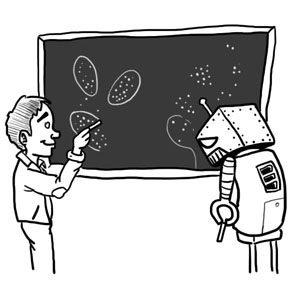
\includegraphics[scale=0.5]{images/clustering_joke.jpg}
\end{center}

\end{frame}

\begin{frame}{Обучение без учителя}

В задачах {\bf без учителя} значение целевой функции для объектов из обучающей выборки неизвестно. Решение таких задач подразумевает исследование ``скрытой структуры'' данных.

\vspace{2em}
Задача {\bf кластеризации} -- задача без учителя, подразумевающая разбиение множества объектов на непересекающиеся подмножества (кластеры).

\end{frame}

\begin{frame}{Мотивация}

\begin{itemize}
\item
\only<1>{Кластеризация позволяет больше узнать о данных (knowledge discovery!)}
\only<2>{Работать с кластерами удобнее, чем c отдельными объектами}
\only<3>{Кластеризация позволяет конструировать новые признаки}
\end{itemize}

\only<1>{
\begin{figure}
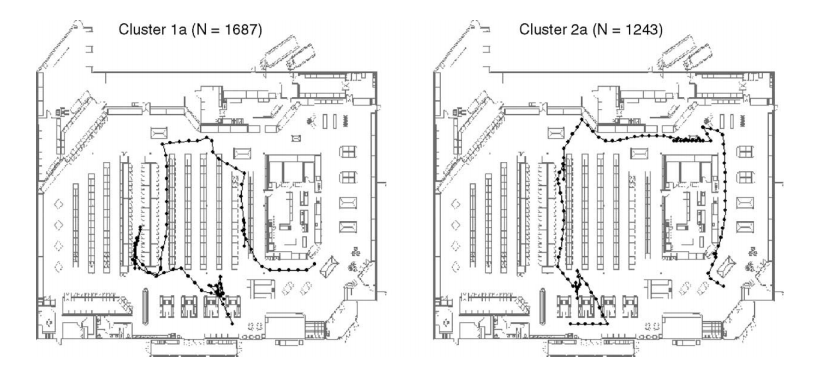
\includegraphics[width=0.8\textwidth]{images/paths.png}
\caption{Типичные траектории покупателей супермаркета\footnote{\href{https://statistics.wharton.upenn.edu/files/?whdmsaction=public:main.file&fileID=346}{An exploratory look at supermarket shopping paths // J.S. Larson et. al.}}}
\end{figure}
}
\only<2>{
\begin{figure}
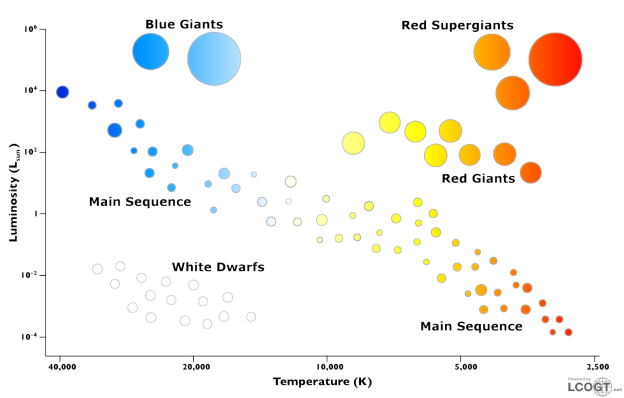
\includegraphics[height=0.55\textheight]{images/hrdiagram.png}
\caption{Диаграмма Герцшпрунга — Рассела\footnote{\url{https://lcogt.net/spacebook/h-r-diagram/}}}
\end{figure}
}
\only<3>{
\begin{quote}
\texttt{d1: Банк финансирует строительство футбольного стадиона} \\
\texttt{d2: Автомобили подорожали из-за финансового кризиса } \\
\end{quote}
\vspace*{\fill}
\begin{tabular}{r | c c c c c c c c c}
& \rot{\it банк} & \rot{\it финансы} & \rot{\it строительство} & \rot{\it футбол} & \rot{\it стадион} & \rot{\it автомобиль} & \rot{\it подорожание} & \rot{\it кризис} & \ldots \\
\hline
\texttt{d1} & 1 & 1 & 1 & 1 & 1 & 0 & 0 & 0 & \ldots \\
\texttt{d2} & 0 & 1 & 0 & 0 & 0 & 1 & 1 & 1 & \ldots \\
& \multicolumn{9}{c}{\ldots}
\end{tabular} \quad \tikzarrow{pink}{clustering} \quad
\begin{tabular}{r | c c c c}
& \rot{\it экономика} & \rot{\it спорт} & \rot{\it производство} & \ldots \\
\hline
\texttt{d1} & 2 & 2 & 1 & \ldots \\
\texttt{d2} & 3 & 0 & 1 & \ldots \\
 & \multicolumn{4}{c}{\ldots}
\end{tabular}
}

\end{frame}

\begin{frame}{Задача кластеризации}

\vspace{1em}
{\bf Дано.} Признаковые описания $N$ объектов $\mathbf{x} = (x_1, \ldots, x_m) \in \mathcal{X}$, образующие тренировочный набор данных $X$

\vspace{1em}
{\bf Найти.} Модель из семейства параметрических функций 
\[
H = \{h(\mathbf{x, \mathbf{\theta}}): \mathcal{X} \times \Theta \rightarrow \mathcal{Y} \mid \mathcal{Y} = \{1, \ldots, K\}\},
\]
ставящую в соответствие произвольному $\mathbf{x} \in \mathcal{X}$ один из $K$ кластеров так, чтобы объекты внутри одного кластера были похожи, а объекты из разных кластеров различались

\end{frame}

% =======================
\section{Смесь нормальных распределений и EM}
% =======================

\begin{frame}{}

\begin{center}
{\LARGE Смесь нормальных распределений и EM}

\vspace{2em}
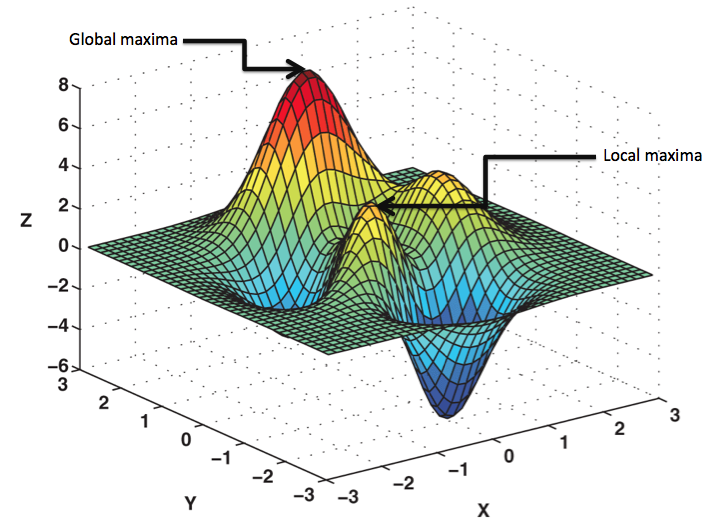
\includegraphics[scale=0.3]{images/local.png}
\end{center}

\end{frame}

\begin{frame}{Начнем с простого (смоделируем один кластер)}

{\bf Данные} \\ Координаты точек попаданий по мишени из гауссовской пушки 

{\bf Задача} \\ Определить, куда смещен прицел

\begin{figure}
	\centering
	 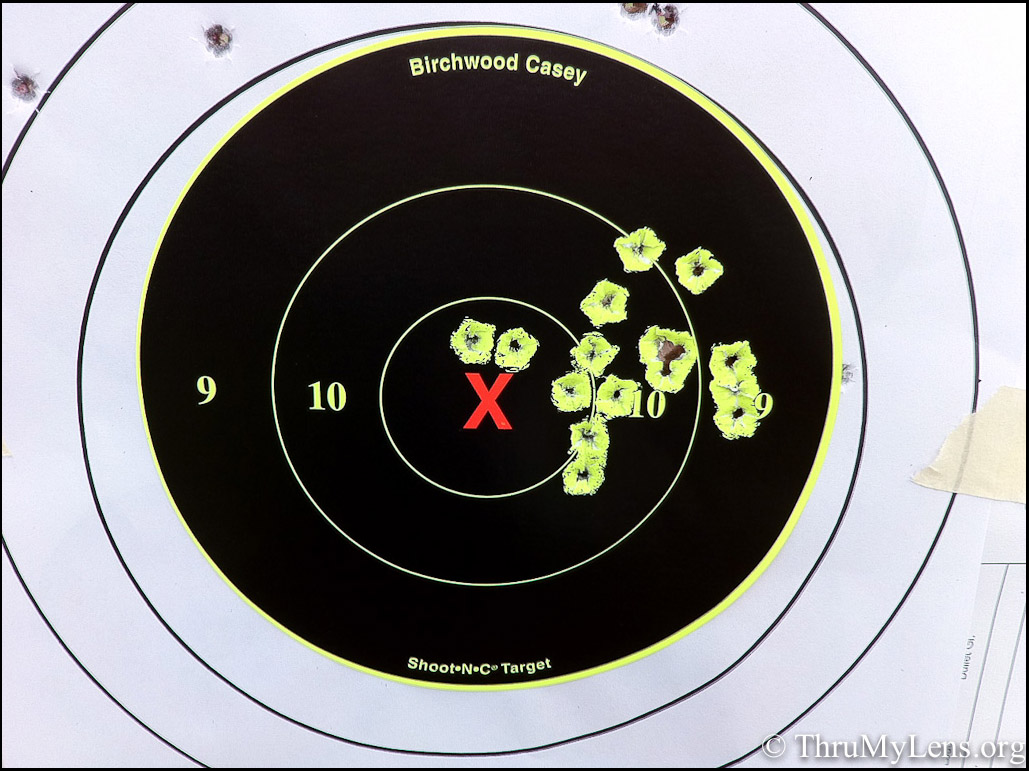
\includegraphics[width=0.5\textwidth]{images/target.jpg}       
\end{figure}

\end{frame}

\begin{frame}{Гаусс, Карл Фридрих (1777-1855)}

\begin{figure}
	\centering  
	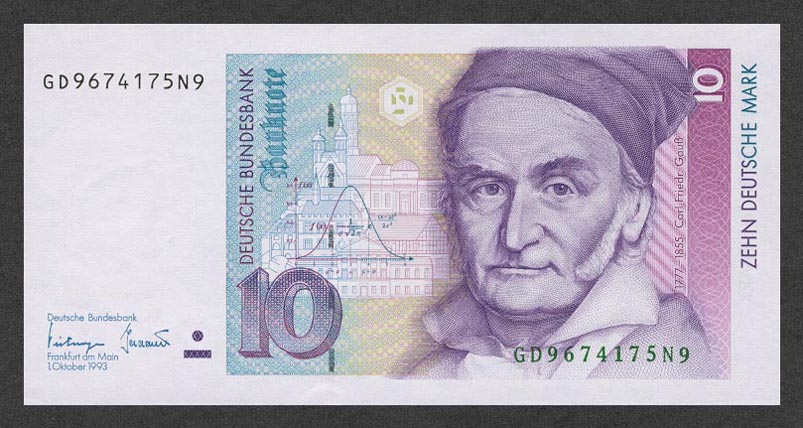
\includegraphics[width=0.8\textwidth]{images/gauss.jpg}
\end{figure}

\begin{itemize}
\item Не открыл распределение Гаусса
\item Открыл все остальное
\end{itemize}

\end{frame}

\begin{frame}{Многомерное нормальное распределение}

\[
\mathcal{N(\mathbf{x} | \mathbf{\mu}, \mathbf{\Sigma}}) = \frac{1}{(2 \pi)^{D/2}} \frac{1}{|\mathbf{\Sigma}|^{1/2}} \exp \left\{-\frac{1}{2}(\mathbf{x} - \mathbf{\mu})^T \mathbf{\Sigma^{-1}} (\mathbf{x} - \mathbf{\mu})\right\}
\]

\vspace{0.7em}
\begin{center}
{\bf Параметры}
\end{center}
\quad${D}$-мерный вектор средних\qquad$D \times D$-мерная матрица ковариации 
\[
\mathbf{\mu} = \int \mathbf{x} p({\mathbf{x}}) d\mathbf{x}
\qquad\qquad\qquad
\mathbf{\Sigma} = E[(\mathbf{x} - \mathbf{\mu})(\mathbf{x} - \mathbf{\mu})^T]
\]
\begin{figure}
        \centering
        \begin{subfigure}[b]{0.23\textwidth}
                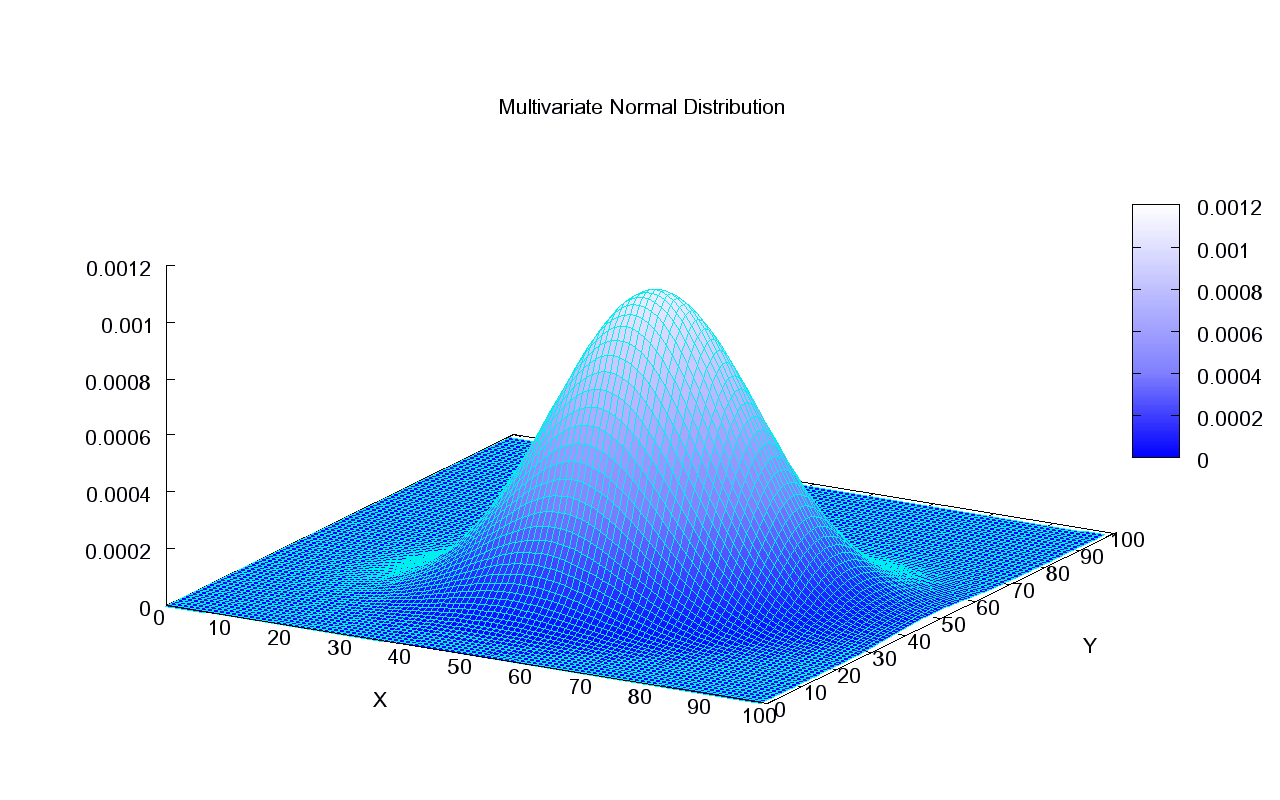
\includegraphics[width=\textwidth]{images/multi.png}
                \caption{$D = 2$}                
        \end{subfigure}    
        \begin{subfigure}[b]{0.23\textwidth}
                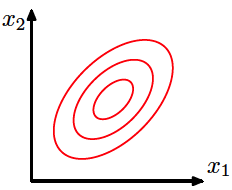
\includegraphics[width=\textwidth]{images/gnormal.png}
                \caption{}     
        \end{subfigure}
        \begin{subfigure}[b]{0.23\textwidth}
                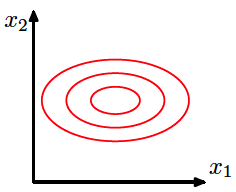
\includegraphics[width=\textwidth]{images/dnormal.png}
                \caption{$\mathbf{\Sigma} = \text{diag}(\sigma_i)$}
        \end{subfigure}
        \begin{subfigure}[b]{0.23\textwidth}
                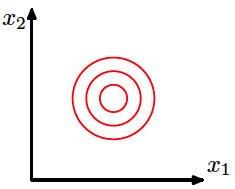
\includegraphics[width=\textwidth]{images/enormal.png}
                \caption{$\mathbf{\Sigma} = \sigma I$}
        \end{subfigure}
\end{figure}

\end{frame}

\begin{frame}{Формализуем задачу}

Имеется набор данных
\[
X = \{\mathbf{x}_n \in R^2\}
\]
Предположение
\[
p(\mathbf{x}_n) \sim \mathcal{N(\mathbf{x} | \mathbf{\mu}, \mathbf{\Sigma}}), \quad \mu \in R^2, \;\; \mathbf{\Sigma} \in R^{2 \times 2}
\]
Требуется найти вектор средних $\mu$ и матрицу ковариации $\mathbf{\Sigma}$

\end{frame}

\begin{frame}{Maximum likelihood (!)}

\begin{block}{Принцип максимального правдоподобия}
Пусть дано семейство параметрических моделей $h(\mathbf{x}, \mathbf{\theta})$. Выбираем вектор параметров $\theta$, максимизирующий функцию правдоподобия (likelihood) $p(\mathcal{D} | \theta)$, соответствующую рассматриваемому семейству моделей.
\end{block}

\vspace{1em}
Правдоподобие
\[
L(X | \mu, \mathbf{\Sigma}) = \prod_{n=1}^N \mathcal{N}(\mathbf{x_n} | \mathbf{\mu}, \mathbf{\Sigma}) \rightarrow \max_{\mu, \mathbf{\Sigma}}
\]
Решение
\[
\mu_{ML} = \frac 1 N \sum_{n=1}^N \mathbf{x_n}, \quad \mathbf{\Sigma}_{ML} = \frac 1 N \sum_{n=1}^N (\mathbf{x_n} - \mu_{ML}) (\mathbf{x_n} - \mu_{ML})^T
\]

\end{frame}

\begin{frame}{Old Faithful data set}

\begin{quote}
D = date of recordings in month (in August) \\
X = duration of the current eruption in minutes \\
Y = waiting time until the next eruption in minutes \\
\end{quote}

\begin{figure}
        \centering
        \begin{subfigure}[b]{0.25\textwidth}
                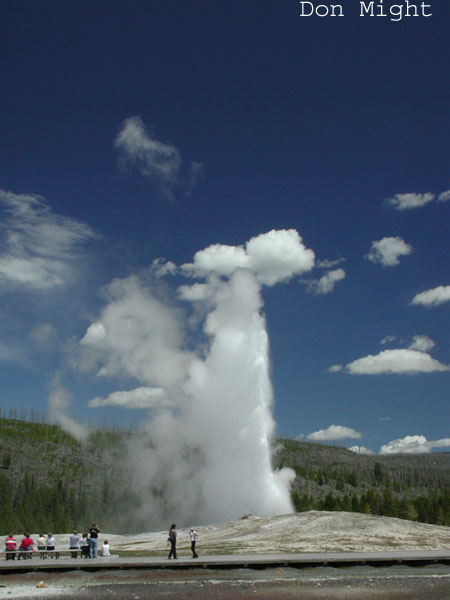
\includegraphics[width=\textwidth]{images/of1.jpg}
                \caption{Yellowstone Park}                
        \end{subfigure}    
        \begin{subfigure}[b]{0.5\textwidth}
                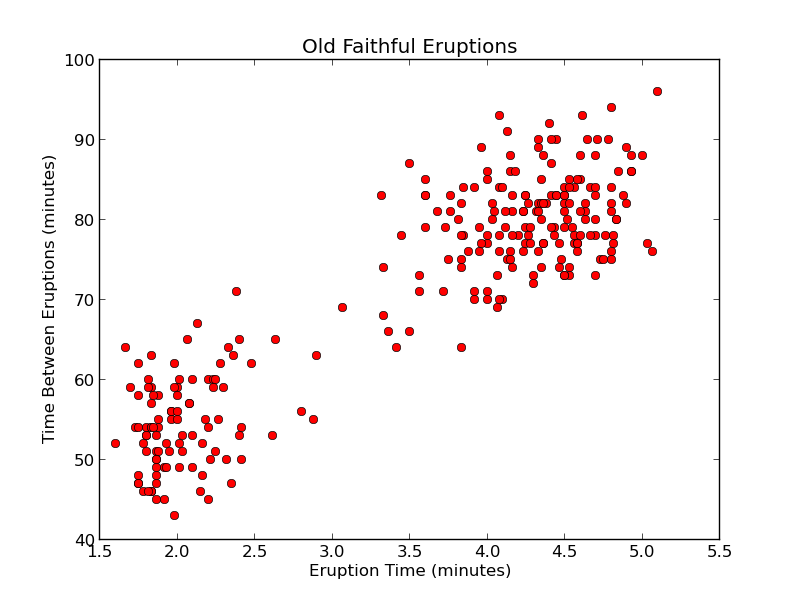
\includegraphics[width=\textwidth]{images/of2.png}
                \caption{}
        \end{subfigure}        
\end{figure}

\end{frame}

\begin{frame}{Смесь нормальных распределений}

``Скрытая'' $K$-мерная переменная $\mathbf{z}$ -- принадлежность объекта к одному из кластеров
\[
p(z_k = 1) = \pi_k, \quad z_k \in \{0, 1\}, \quad \sum_k z_k = 1 \quad\rightarrow\quad p(\mathbf{z}) = \prod_k \pi_k^{z_k}
\]

Распределение $\mathbf{x}$ для каждого из $K$ кластеров
\[
p(\mathbf{x} | \mathbf{z_k}) = \mathcal{N}(\mathbf{x} | \mathbf{\mu}_k, \mathbf{\Sigma}_k) \quad \rightarrow \quad p(\mathbf{x} | \mathbf{z}) = \prod_k \mathcal{N}(\mathbf{x} | \mathbf{\mu}_k, \mathbf{\Sigma}_k)^{z_k}
\]
Смесь нормальных распределений
\[
p(\mathbf{x}) = \sum_k \pi_k \mathcal{N}(\mathbf{x} | \mathbf{\mu}_k, \mathbf{\Sigma}_k)
\]

\end{frame}

\begin{frame}{}

Апостериорная вероятность принадлежности к $k$ кластеру (априорная равна $\pi_k$)
\[
\gamma(z_k) = p(z_k = 1 | \mathbf{x}) = \frac{p(z_k=1) p(\mathbf{x} | z_k = 1)}{\sum_{j=1}^K p(z_j=1) p(\mathbf{x} | z_j = 1)} =
\]
\[
= \frac{\pi_k \mathcal{N}(\mathbf{x} | \mathbf{\mu}_k, \mathbf{\Sigma}_k)}{\sum_{j=1}^K \pi_j \mathcal{N}(\mathbf{x} | \mathbf{\mu}_j, \mathbf{\Sigma}_j)}
\]

\end{frame}

\begin{frame}{Maximum Likelihood}

Функция правдоподобия
\[
\log(\mathbf{X} | \mathbf{\pi}, \mathbf{\mu}, \mathbf{\Sigma}) = \sum_{n=1}^N \log \sum_k \pi_k \mathcal{N}(\mathbf{x}_n | \mathbf{\mu}_k, \mathbf{\Sigma}_k) \rightarrow \max_{\mathbf{\pi}, \mathbf{\mu}, \mathbf{\Sigma}}
\]

Сложности
\begin{itemize}
\item схлопывание компонент
\item переименование кластеров
\item невозможно оптимизировать аналитически
\end{itemize}

\end{frame}

\begin{frame}{}

Дифференцируем функцию правдоподобия
\[
N_k = \sum_{n=1}^N \gamma(z_{nk}), \;\; \mu_k = \frac 1 {N_k} \sum_{n=1}^N \gamma(z_{nk}) \mathbf{x}_n
\]
\[
\Sigma_k = \frac 1 {N_k} \sum_{n=1}^N \gamma(z_{nk}) (\mathbf{x}_n - \mu_k)^T (\mathbf{x}_n - \mu_k)
\]
\[
\pi_k = \frac{N_k}{N}
\]

\end{frame}

\begin{frame}{Expectation Maximization (!)}

\begin{enumerate}
\item[E] Expectation: при фиксированных $\mu_k, \Sigma_k, \pi_k$
\[
\gamma(z_{nk}) = \frac{\pi_k \mathcal{N} (\mathbf{x}_n | \mu_k, \Sigma_k)}{\sum_{j=1}^K \pi_j \mathcal{N} (\mathbf{x}_n | \mu_j, \Sigma_j)}
\]
\item[M] Maximization: при фиксированных $\gamma(z_{nk})$
\[
N_k = \sum_{n=1}^N \gamma(z_{nk}), \;\; \mu_k = \frac 1 {N_k} \sum_{n=1}^N \gamma(z_{nk}) \mathbf{x}_n
\]
\[
\Sigma_k = \frac 1 {N_k} \sum_{n=1}^N \gamma(z_{nk}) (\mathbf{x}_n - \mu_k)(\mathbf{x}_n - \mu_k)^T
\]
\[
\pi_k = \frac{N_k}{N}
\]
\item[S] Остановиться при достижении сходимости
\end{enumerate}

\end{frame}

\begin{frame}{}

\begin{center}
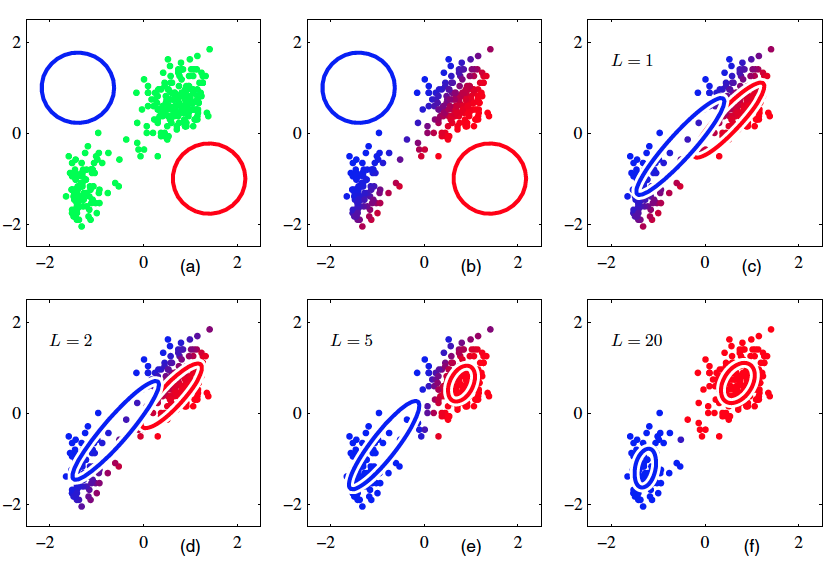
\includegraphics[scale=0.35]{images/gauss.png}
\end{center}

\end{frame}

\begin{frame}{EM-алгоритм\footnote{\href{http://web.mit.edu/6.435/www/Dempster77.pdf}{Maximum Likelihood from Incomplete Data via the EM Algorithm}}}

{\bf Дано.} \\ Известно распределение $P(\mathbf{X}, \mathbf{Z} | \theta)$, где $\mathbf{x}$ -- наблюдаемые переменные, а $\mathbf{z}$ -- скрытые. 

{\bf Найти.} \\ $\theta$,  максимизирующее $P(\mathbf{X} | \theta)$.

\vspace{1em}
\begin{itemize}
\item[E] вычислить $P(\mathbf{Z} | \mathbf{X}, \theta^{old})$ при фиксированном $\theta^{old}$
\item[M] вычислить $\theta^{new} = \arg \max_{\theta} \mathcal{Q} (\theta, \theta^{old})$, где
\[
\mathcal{Q} (\theta, \theta^{old}) = E_\mathbf{Z}[\ln p(\mathbf{X}, \mathbf{Z} | \theta)] = \sum_{\mathbf{Z}} p(\mathbf{Z} | \mathbf{X}, \theta^{old}) \ln p(\mathbf{X}, \mathbf{Z} | \theta))
\]
\end{itemize}
{\it Улучшение:} ввести априорное распределение $p(\theta)$

\end{frame}

\begin{frame}{Сходимость\footnote{\href{http://www.cs.cmu.edu/~dgovinda/pdf/recog/EM_algorithm-1.pdf}{The Expectation Maximization Algorithm: A short tutorial}}}

\begin{center}
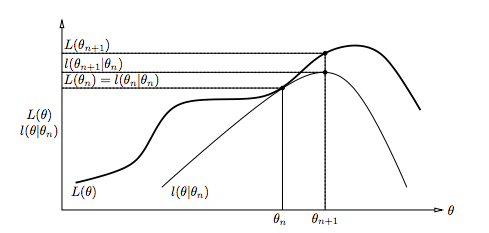
\includegraphics[scale=0.6]{images/convergence.png}
\end{center}

\end{frame}

\begin{frame}{Различные смеси}

\begin{center}
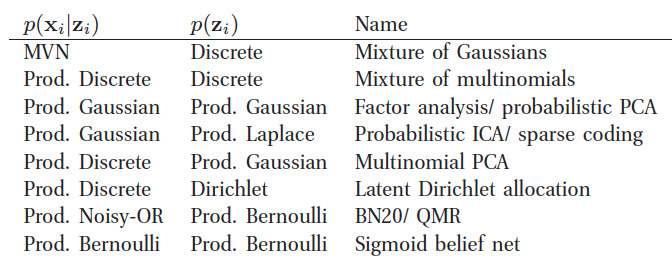
\includegraphics[scale=0.4]{images/mixtures.png}
\end{center}

\end{frame}

% =======================
\section{K-means и его модификации}
% =======================

\begin{frame}{}

\begin{center}
{\LARGE K-means и его модификации}

\vspace{2em}
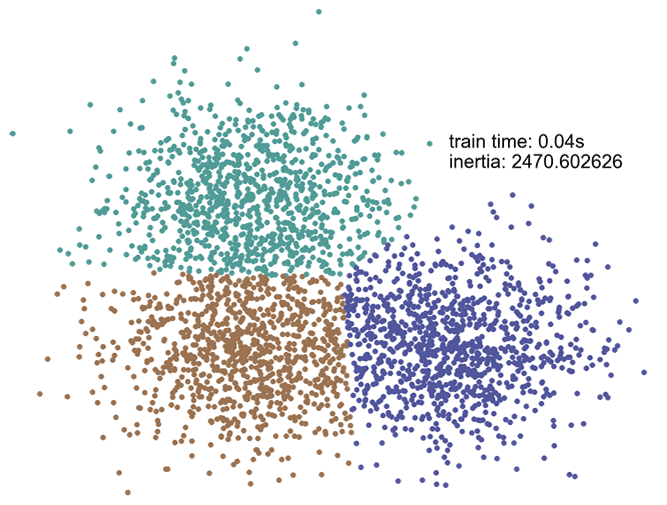
\includegraphics[scale=0.3]{images/k-cover.png}
\end{center}

\end{frame}

\begin{frame}{K-means}

Пусть $\Sigma_k = \epsilon I$, тогда
\[
p(\mathbf{x} | \mu_k, \Sigma_k) = \frac{1}{\sqrt{2\pi\epsilon}}\exp(-\frac{1}{2\epsilon}\|\mathbf{x}-\mathbf{\mu_k}\|^2)
\]
Рассмотрим стремление $\epsilon \rightarrow 0$
\[
\gamma(z_{nk}) = \frac{\pi_k \exp(-\frac{1}{2\epsilon}\|\mathbf{x}_n-\mathbf{\mu_k}\|^2)}{\sum_j \pi_j \exp(-\frac{1}{2\epsilon}\|\mathbf{x}_n-\mathbf{\mu_j}\|^2)} \rightarrow r_{nk} = \begin{cases}
1, \; \text{для } k = \arg \min_j \|\mathbf{x}_n - \mathbf{\mu_j}\|^2 \\
0, \; \text{иначе}
\end{cases}
\]
Функция правдоподобия
\[
E_\mathbf{Z}[\ln p(\mathbf{X}, \mathbf{Z} | \mu, \Sigma, \pi)] \rightarrow -\sum_{n=1}^N \sum_{k=1}^K r_{nk} \| \mathbf{x}_n - \mu_k \|^2 + const
\]
Вектор средних
\[
\mathbf{\mu}_k = \frac{\sum_n r_{nk} \mathbf{x_n}}{\sum_n r_{nk}} 
\]

\end{frame}

\begin{frame}{K-means}

\kmeans
Сложность $O(NK)$ \\
Локальная оптимизация (!)

\end{frame}

\begin{frame}{}

\begin{center}
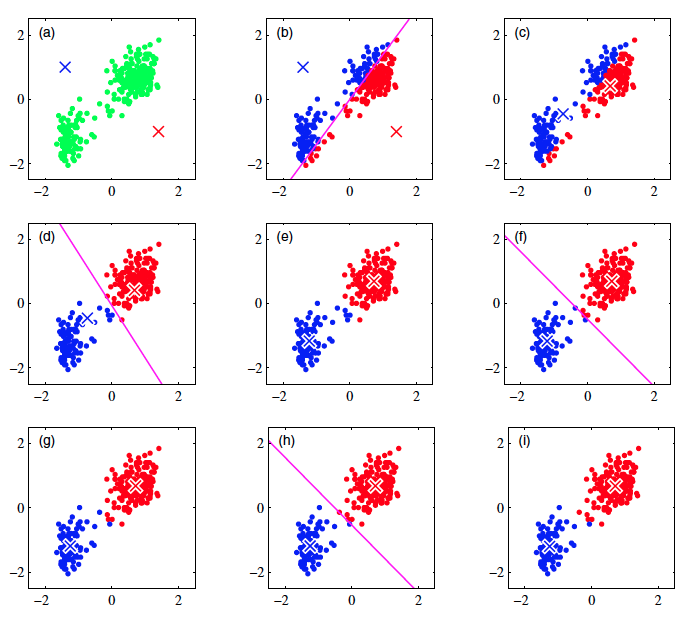
\includegraphics[scale=0.35]{images/kmeans.png}
\end{center}

\end{frame}

\begin{frame}{Задача}

\begin{center}
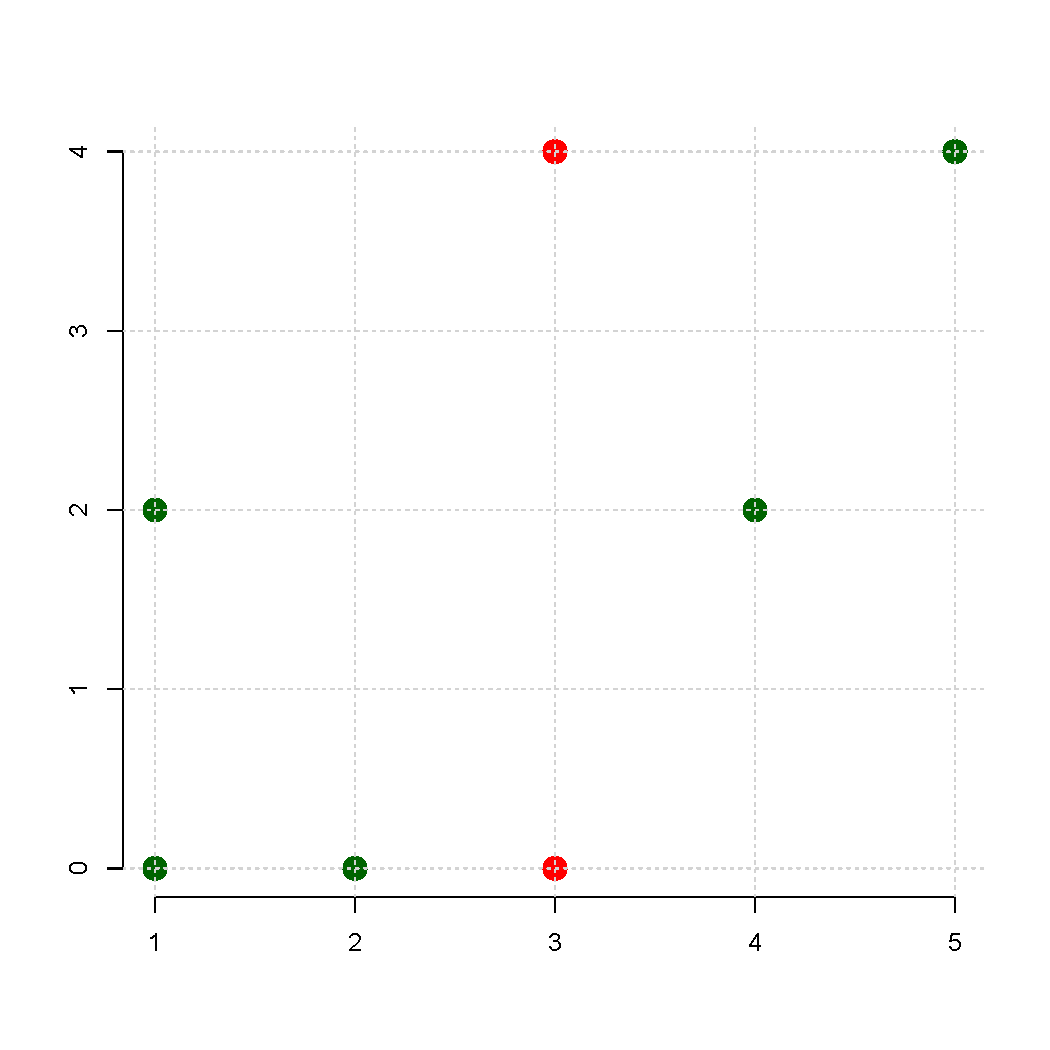
\includegraphics[height=0.9\textheight]{images/problem.pdf}
\end{center}

\end{frame}

\begin{frame}{Модификации k-means (1)}

\begin{itemize}
\item На каждом шаге работаем с $b$ случайно выбранными объектами из каждого кластера (mini-batch k-means) \\
\begin{center}
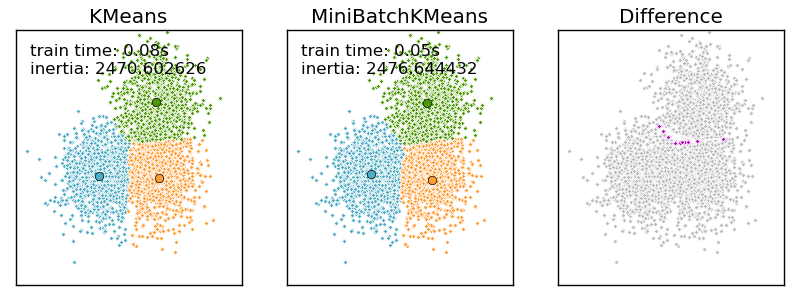
\includegraphics[scale=0.35]{images/mbatch.png}
\end{center}
\item Критерий качества (k-medoids)
\[
\tilde J = \sum_{n=1}^N \sum_{k=1}^K r_{nk} d(\mathbf{x}_n, \mu_k)
\]
$d$ -- функция расстояния, $\mu_k$ -- один из объектов в кластере
\end{itemize}

\end{frame}

\begin{frame}{Модификации k-means (2)}

\begin{itemize}
\item k-means++ -- ``умная'' инициализация\footnote{\href{http://theory.stanford.edu/~sergei/papers/kMeansPP-soda.pdf}{k-means++: The Advantages of Careful Seeding}}
\item онлайн k-means
\[
\mu_k^{new} = \mu_k^{old} + \eta_n (\mathbf{x}_n - \mu_k^{old})
\]
\end{itemize}

\end{frame}

\begin{frame}{Кластеризация}

\begin{block}{Идея}
Выбрать критерий качества кластеризации $J$ и расстояние между объектами $d(\mathbf{x}_i, \mathbf{x}_j)$ и вычислить разбиение выборки на кластеры, которое которое соответствует оптимальному значению выбранного критерия.
\end{block}

\end{frame}

\begin{frame}{Альтернативные критерии качества}

Критерий
\begin{eqnarray*}
J &=& \sum_{k=1}^K \sum_{\mathbf{x}_i \in C_k} \| \mathbf{x}_i - \mathbf{m}_k \|^2 = \\
&=& \frac 1 2 \sum_{k=1}^K n_k \left[ \frac{1}{n_k^2} \sum_{\mathbf{x}_i \in C_k} \sum_{\mathbf{x}_j \in C_k} \| \mathbf{x}_i - \mathbf{x}_j \|^2 \right] = \\
&=& \frac 1 2 \sum_{k=1}^K n_k \left[ \frac{1}{n_k^2} \sum_{\mathbf{x}_i \in C_k} \sum_{\mathbf{x}_j \in C_k} s(\mathbf{x}_i, \mathbf{x}_j) \right] = \frac 1 2 \sum_{k=1}^K n_k \bar s_k
\end{eqnarray*}
Примеры $\bar s_i$
\[
\underline{s}_k = \min_{\mathbf{x}_i, \mathbf{x}_j} s(\mathbf{x}_i, \mathbf{x}_j); \quad \bar s_k = \max_{\mathbf{x}_i, \mathbf{x}_j} s(\mathbf{x}_i, \mathbf{x}_j)\]

\end{frame}

\begin{frame}{Задача на дом}

Рассмотреть смесь из $D$-мерных распределений Бернулли. В такой смеси $\mathbf{x}$ -- $D$-мерный бинарный вектор, каждый компонент $x_i$ которого подчиняется распределению бернулли с параметром $\mu_{ki}$ при заданном векторе $\mu_k$:
\[
p(\mathbf{x} | \mu_k) = \prod_{i=1}^D \mu_{ki}^{x_i} (1-\mu_{ki})^{(1-x_i)}
\]
Вероятность $k$-го вектора $\mu_k$ равна $\pi_k$. Выписать выражения для E и M шагов при исользовании EM алгоритма для нахождения неизвестных параметров $\mu_k$ и $\pi_k$.

\end{frame}

\begin{frame}[plain]
\begin{center}
{\Large Вопросы}
\end{center}
\end{frame}

\end{document}